\chapter{Implementation of Dynamic Graph Tracking in Julia}
\label{cha:impl-dynam-graph}

It has been described above that there is a trade-off between source-transformation methods and
library-based (operator overloading) approaches for tracking computation graphs.  Since the ultimate
goal of this work was to analyze dynamic probabilistic models written in \turingjl{}, properties of
both were derired.  Operator overloading has been considered as well, since it would have allowed to
potentially reuse AD implementations, but was thought insufficient, because the structure of control
flow and recursion are lost.  Inspired the the work of \textcite{innes2018don}, it seemed most
promising to start from a source-transformation based approach implemented over the intermediate
representation, especially from a usability point of view.  The advantages of using a transformation
of the IR over the surface AST are the same: there is less overhead from handling multiple syntactic
forms, and naming is already referentially transparent.  Additionally, there are existing Julia
packages to simplify handling the IR data structures and set up the transformations.

However, the dynamicity of the trace structure of general probabilistic programs needs to be
preserved and exposed to the user, for each function evaluation~-- which is different from the AD
usage, where the adjoint function is already the ultimate goal, and does not change with the
arguments.  Hence, a method for a hybrid version was developed: through an IR transformation, the
original code of a function to be tracked should be exteded by additional statements to record a
trace of the executed statements and control flow operations at runtime.  The algorithm and data
structure on which this approach is based have already been shortly described in
\textcite{gabler2019graph}, and will be more extensively explained below.  An open source
implementation is available
online\footnote{\protect\url{https://github.com/TuringLang/IRTracker.jl}}.

As we have seen above, in section~\ref{sec:comp-metapr-julia}, generated functions allow the
inspection and transformation of the intermediate representation passed-in functions.  This
technique can be applied to recursively traverse the implementation of a given function, annotating
each operation with necessay tracking statements, and changing the inputs and outputs accordingly to
extract this information from outside.  To ensure sufficient generality, we requite the following
properties of the tracking system:
\begin{enumerate}
  \firmlist
\item Storage of all intermediate values during execution.
\item Symbolic capture expressions and branches in an analyzable, graphical form.
\item Preservation of the relation of each part of the structure to the corresponding original IR.
\item Proper nesting of this information for nested function calls, making relations between
  arguments and function inputs recoverable.
\item Correct handling of constants and primitive functions in the IR.
\item Extensibility of the tracking functions, to allow multiple possible ways to analyze code
  (e.g., by different definitions of what should be recorded).
\item A way to add custom metadata to the recorded structure during tracking.
\end{enumerate}
This kind of operation will be similar to the (explicit) construction of Wengert lists in
backwards-mode AD (see section~\ref{sec:cg-ad}); but contrary to there, the nested call structure
and control flow shall be preserved as well.  Hence, we call this structure \emph{extended Wengert
  list}.  

\section{Extended Wengert Lists}
\label{sec:exteded-wengert-lists}

The extended Wengert list structure is implemented in Julia through nested objects of an abstract
supertype \jlinl{AbstractNode}, with several concrete subtypes for the different kinds of nodes.
Additionally, there are special types for the tape- and block references, and an expression type
\jlinl{TapeExpression}, mimicking the built-in \jlinl{Expr}, but adding more semantic distinctions
(such as between references and constants, and between primitive and non-primitive function calls).
On top of this, an API to query the graph structure is provided, allowing, for example, to find all
children or parents of a tape refererence up to a certain depth, or extract data from nodes, such as
referenced variables, arguments, or metadata.

\begin{figure}[t]
  \centering
  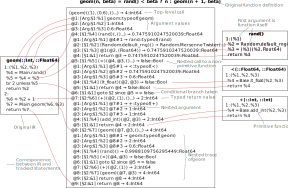
\includegraphics[width=\textwidth]{figures/extended-wengert-list}
  \caption{Extended Wengert list for one run of the stochastic function geom (only three levels
    shown). The central box is the tracked graph of the call \protect\jlinl{geom(1, 0.6)}. The other
    boxes show the original IR of the called non-primitive functions, to which the nodes are
    linked.  Angle brackets indictate constant values.}
  \label{fig:ext-wengert-list}
\end{figure}

Figure~\ref{fig:ext-wengert-list} illustrates the resulting extended Wengert list for one run of a
short stochastic function:
\begin{lstlisting}
geom(n, beta) = rand() < beta ? n : geom(n + 1, beta)
\end{lstlisting}
(for readability, the result is displayed to only three levels of nesting).  The function draws a
sample from the geometric distribution with parameter \jlinl{beta}, starting to count at value
\jlinl{n}. On the left, we have its IR in textual form, consisting of two blocks. The central part
is the graph of nested nodes.  There, values and jumps from the top-level call are recorded in their
encountered order, as nodes with \enquote{tape references} \jlinl{@1} to \jlinl{@9}. SSA variables
(\jlinl{\%i}) occurring in expressions of SSA definitions are also replaced in the nodes by the
respective tape references.  Each node is linked to the original IR statement it records, as
indicated by the red arrows.

In the lower middle part, we see the node corresponding to the statement \jlinl{\%7 = geom(\%6,
  \%3)}.  It is recorded at reference \jlinl{@8} with expression \jlinl{geom(@7, @3)} and value
\jlinl{4} (the notation \jlinl{⟨geom⟩(@7, @3, ()...)} indicates that \jlinl{geom} is a constant, and
no variadic arguments are passed). The values of the arguments of this call can be inspected by
looking up the respective references.  Since \jlinl{geom} is not a primitive function, the node
holds tape of child nodes as well.  In this case, it is equivalent to the top level, due to the
recursivity of \jlinl{geom}. We can see the three arguments \jlinl{@1}, \jlinl{@2}, and \jlinl{@3},
corresponding to the block arguments \jlinl{\%1}, \jlinl{\%2}, and \jlinl{\%3}, with the value of
\jlinl{@2} being now \jlinl{2} instead of \jlinl{1}.  Further we can see function calls of
\jlinl{rand} and \jlinl{<} as well as a conditional jump, corresponding to the branch the original
IR, followed by calls of \jlinl{+} and \jlinl{geom}. Following back the tape references from the
result value \jlinl{@9}, the data path of the trace can be extracted.  It can be used for
reverse-mode AD, and only these nodes would be recorded in a conventional Wengert list.  In this
work, however, the system also records the nodes on the control path, consisting of \jlinl{@6} and
the nodes it depends on.


\section{Automatic Graph Tracking}
\label{sec:autom-graph-track}

Recording an extended Wengert list requires to capture all block arguments, SSA definitions, and
taken branches, with their actual values and metadata. This is achieved by extending the IR with new
statements creating nodes and recording them on the extended Wengert list structure described in the
previous section. Care needs to be taken to properly record function calls, since we need to ensure
that non-primitive functions are recursively tracked.

The recording functionality is implemented as a transformation using a generated function operating
on the IR, using the \juliapackage{IRTools.jl} package, as described in
section~\ref{sec:comp-metapr-julia}.  The resulting IR consists of about three to five times as many
statements as the original.  The basic blocks and control structure are preserved, except for the
redirection of return statements to the one block at the end.  Due to JIT compilation, the
transformation is performed at most a constant number of times per method, and then stored as
compiled code.  However, the tracking~-- the recording of all statements in the extended Wengert
list structure~-- happens at every execution during runtime.  Furthermore, the extended code is
available to all standard optimizations performed in the following passes of type inference and
lowering.

The transformed code of the example function \jlinl{geom}, whose IR is displayed in
figure~\ref{fig:ext-wengert-list} above, is displayed in figure~\ref{fig:geom-tracked}.  First, a
\enquote{graph recorder} object is passed into the function via the extra argument \jlinl{\%5}.  In
this, the original IR is stored for later access.  Subsequently, every original SSA statement is
replaced by a call to one of the \protect\jlinl{trackedX} functions, to which both the function and
its arguments, wrapped into \jlinl{TapeExpression}s directly (for constants) or indirectly (through
\jlinl{trackedvariable} and \jlinl{trackedargument}, which preserve the symbolic mapping to SSA
variables).  The \jlinl{record!}  function takes care of constructing the child node of the possibly
nested call, and storing them on the recorder object.

\begin{figure}[p]
  % \hrule
  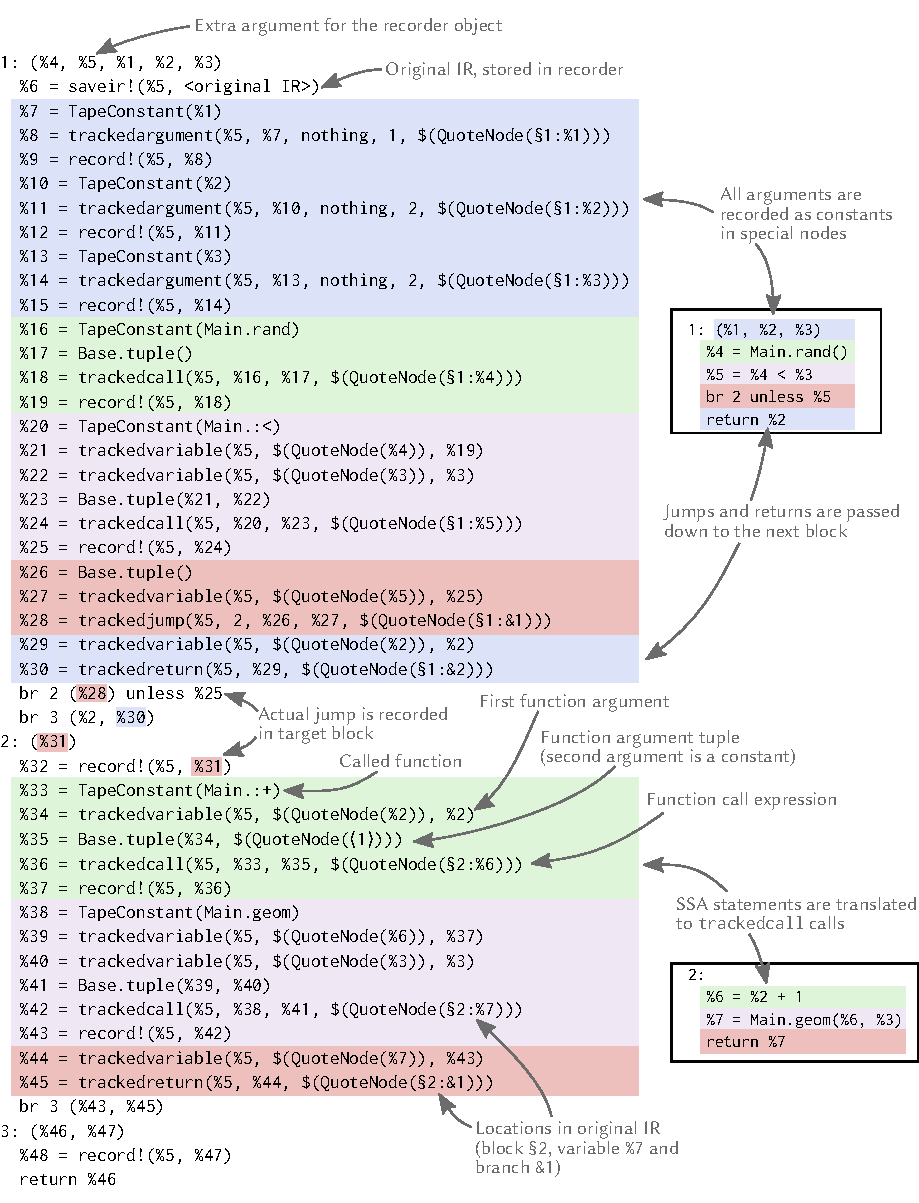
\includegraphics[width=\textwidth]{figures/translation}
  % \hrule
  \caption{Tracked IR of the method \protect\jlinl{geom(::Int, ::Float64)}.  Corresponding parts in
    original and transformed IR are highlighted in matching colors.  (The original IR consists of
    two blocks, shown separately on the right.)\label{fig:geom-tracked}}
\end{figure}
\todo{make sure figure is on same spread as explanation}

To get a more detailed understanding, consider the SSA statement \jlinl{\%6 = \%2 + 1} in the second
block, which describes the application of the function \jlinl{+} to an SSA variable and a constant.
The corresponding transformed IR is shown in the lower part of the figure, highlighted in green.
\begin{enumerate}
  \firmlist
\item First, a constant node \jlinl{\%33} for the function is set up.
\item Then, the variable argument in is tracked in \jlinl{\%34}.  There, \jlinl{trackedvariable} has
  the purpose to correctly relate the node in the trace (\jlinl{@2}) to the original SSA variable
  \jlinl{\%6}.  This is necessary since a block could be visited multiple times during tracking~--
  for example, if it belongs to a loop body~-- which requires to give multiple, unique names to
  references to the same original variable.  Additionally, \jlinl{trackedvariable} copies values,
  since the tracked information would otherwise no preserve intermediate values correctly in the
  case of mutations.
\item Next, both of the function arguments are packed into the tuple \jlinl{\%35}; the second
  argument, which was a literal value \jlinl{1} in the original IR, is preserved as a literal as
  well (wrapped into a \jlinl{QuoteNode} object for technical reasons).
\item Finally, the function and arguments are passed to the function \jlinl{trackedcall}, which
  takes care of acually calling the original function.  Doing so, it will, if the called function is
  not considered primitive, recursively track it as well, and pack the resulting child nodes into a
  new nested node, together with the return value.  Otherwise, the result will simply be stored in a
  special primitive-call node.
\item The resulting node is then stored on the recorder; this operation at the same time returns the
  value, \jlinl{\%37}, which is needed in subsequent calculations (in this case, in \jlinl{\%39}, as
  the argument of the recursive call to \jlinl{geom}).
\end{enumerate}
Branches, tracked with \jlinl{trackejump} and \jlinl{trackedreturn}, cannot be stored on the
recorder object before the respective jumps are taken.  The solution is to first construct the
respective nodes of all possible branches of a block (e.g., \jlinl{\%28}), and adding them as an
extra argument to the old branches.  Then, in each target branch, the jump node from which the
branch originated is recorded immediately (in this case, in statement \jlinl{\%32}).  As a special
case, all return branches are converted to unconditional jumps to one new block at the end, which
contains a single unified return statement (\jlinl{\%30} and \jlinl{\%48} in our example; the branch
variables of block 1 are highlighted in colors matching to the original branches).  This way, return
branches can be treated in the same way as internal branches.  An more formal description in
pseudo-code is given in algorithm~\ref{alg:ir-transform}.

Lastly, some special dispatch is used for the transformation to work correctly on certain special
kinds of function calls, such as built-in functions, type application, and \texttt{ccall}
primitives, which require more careful handling.

\begin{algorithm}[p]
  \footnotesize
  % fix https://github.com/wg030/jlcode/issues/28
  \settowidth{\jlinlem}{\jlinlfont{m}}
  \hrule
  \smallskip
  \begin{algorithmic}
    \Procedure{TransformIR}{\texttt{original\_ir}}
    %
    \State Initialize empty IR object \jlinl{new_ir}
    \Statex
    %
    \For{\jlinl{old_block} in \jlinl{blocks(original_ir)}}
    \State Add an empty block \jlinl{new_block} to \jlinl{new_ir}
    % 
    \If{this is the first block}
    \State Add set up for \jlinl{\%recorder}
    \EndIf
    %
    \Statex
    \LineComment{Handle arguments}
    \State Copy all arguments from \jlinl{old_block} to \jlinl{new_block}
    \State Add tracking and recording for each argument
    %
    \Statex
    \LineComment{Take care of branch recording in target blocks}
    \If{there exist branches to \jlinl{old_block}}
    \State Add new argument \jlinl{\%branch_node} to \jlinl{new_block}
    \State Add recording for \jlinl{\%branch_node}
    \EndIf
    %
    \Statex
    \LineComment{Transform all statements}
    \For{\jlinl{stmt} in \jlinl{statements(old_block)}}
    \State Add tracking and recording for \jlinl{stmt} to \jlinl{new_block}
    \EndFor
    %
    \Statex
    \LineComment{Transform all branches}
    \For{\jlinl{branch} in \jlinl{branches(old_block)}}
    \If{\jlinl{branch} is a return branch}
    \State Add tracking for a return node corresponding to \jlinl{branch}
    \State Add a branch replacing the original return
    \State Pass the original return value and the return node as branch arguments
    \Else
    \State Add tracking statement for a branch node corresponding to \jlinl{branch}
    \State Copy the original \jlinl{branch}
    \State Pass the branch node as extra argument to the branch
    \EndIf
    \EndFor
    %
    \EndFor
    %
    \Statex
    \LineComment{Set up return block}
    \State Add new block to \jlinl{new_ir}, with  arguments \jlinl{\%return_value} and \jlinl{\%return_node}
    \State Add recording of \jlinl{\%return_node}
    \State Add return branch, returning \jlinl{\%return_value} and \jlinl{\%recorder}
    %
    \EndProcedure
  \end{algorithmic}
  \smallskip
  \hrule
  \caption[IR transformation to record an extended Wengert list]{Overview of the IR transformation
    to record an extended Wengert list.  This transformation happens inside a generated function
    called by \protect\jlinl{trackcall}, which assembles the resulting value and IR into a new node
    with the correct metadata.  The details of statement tracking and branch transformation are
    explained in the text; the description of metadata recording, and the mechanisms to correctly
    rename SSA variables during the transformation and tape references at runtime were left out for
    simplicity.\label{alg:ir-transform}}
\end{algorithm}

To provide some modularity and extensibility to the system, it also affords customization of some
behaviour by \emph{tracing contexts}.  All of the \jlinl{trackedX} functions explained above, used
directly in the transformed code, are really special methods that work directly on the recorder
object.  Their behaviour~-- namely, performing the actual method calls and constructing the nodes~--
is defined in another method of the same function, which dispatches on a context object stored in
the recorder object, and can be overloaded by the user for a custom context.  

\begin{lstfloat}
\begin{lstlisting}[style=lstfloat]
struct DepthLimitContext <: AbstractTrackingContext
    level::Int
    maxlevel::Int
end

DepthLimitContext(maxlevel) = DepthLimitContext(1, maxlevel)
canrecur(ctx::DepthLimitContext, f, args...) = ctx.level < ctx.maxlevel

function trackednested(ctx::DepthLimitContext, f_repr::TapeValue,
                       args_repr::ArgumentTuple{TapeValue}, info::NodeInfo)
    new_ctx = DepthLimitContext(ctx.level + 1, ctx.maxlevel)
    return recordnestedcall(new_ctx, f_repr, args_repr, info)
end
\end{lstlisting}
  \caption{Implementation of a tracking context to limit the nesting depth to a maximum (which is
    part of the implemented package).\label{lst:depthlimitcontext}}
\end{lstfloat}

This allows, for one, to overload the notion of what constitutes a \emph{primitive function}.  In
the default context, primitive functions are only those that do not have IR on their own (such as
intrinsics and functions defined in C), which leads to very large recursive traces.  To circumvent
this, we can introduce a new \jlinl{DepthLimitContext}, as shown in
listing~\ref{lst:depthlimitcontext}.  There, the function \jlinl{canrecur} is overloaded to stop at
depth \jlinl{maxlevel}; this method will be called to determine whether a tracked function is
considered primitive.  Besides this, we also have to redefine the behaviour of \jlinl{trackednested}
to specify that for non-primitive functions, i.e., nested calls, the level remembered in the context
object should be updated.  \jlinl{recordnestedcall} is a built-in function of the library that
simply performs the recursive tracking, then.

From this we see that \jlinl{trackedcall} is only a thin wrapper around a conditional statement over
\jlinl{canrecur}, \jlinl{trackednested}, and its sibling \jlinl{trackedprimitive}.  Beyond this,
context dispatch allows a user to change any other of the tracking functions as well.  This can be
used to store custom metadata, calculate information during tracking, or even change return values
or nesting dynamically.  In addition to those methods, also \jlinl{trackedargument},
\jlinl{trackedreturn}, and \jlinl{trackedjump} can be customized, which we have seen in the example;
furthermore, there are \jlinl{trackedspecial}, \jlinl{trackedconstant}, and \jlinl{trackederror}.
\jlinl{trackedvariable} is more primitive and cannot be overloaded, since this would change the
relation between references of tracked nodes.  More information is available on the package's public
repository.

\section{Evaluation}
\label{sec:irtracker-eval}

The extended Wengert list created by tracking a function can be used for many purposes in which
computation graphs are required.  All algorithms that can be formulated as message-passing can
directly work on this, as well as all methods that operate on runtime dependency graphs, from simple
debugging to concolic execution (see discussion below).

As a proof of concept, a small backward-mode AD system was implemented in the form of a context.
This simply required storing the derivative operators for all intermediate values during the forward
pass, and writing a backward pass as graph traversal on the resulting computation
graph.\footnote{\href{https://github.com/TuringLang/IRTracker.jl/blob/760143734de1bf4e90da655d833e7999fc0ab2de/test/test_backward_ad.jl}{\url{https://github.com/TuringLang/IRTracker.jl/blob/master/test/test_backward_ad.jl}}}
The implementation has been tested on some simple composed functions, but is not intended for
serious application.  Due to the very abstract nature of the implemetation, not more individual
evaluations of it are performed, except unit tests to ensure basic correctness of the interface.
The system developed in chapter~\ref{cha:graph-track-prob} provides a larger \enquote{integration
  test}, though.

More potential use cases arise when the tracked model is actually static~-- in this case, the
complete struture can be recovered from one graph tracking pass.  This can then be analyzed and used
in various ways; even more so, when more semantic knowledge about the model exists, such as meanings
of certain domain-specific functions.  Specifically, two show-cases for the system, applied to
probabilistic programs written in \turingjl{} were considered: conjugacy detection as described by
\textcite{hoffman2018autoconj}, and Rao-Blackwellization as in \textcite{murray2017delayed}.  Due to
the additional complexity required for them, only the automatic derivation of Gibbs conditionals, as
shown in the next chapter, was finally executed, though.

The implementation is limited in two respects.  First, in practical terms, there is are some
trade-offs to be made regarding the storage of intermediate results and functions in nodes.  In the
current design, nodes are parametrized by the types of their contents, which leads to very large
types, and potential slow done during type inference.  Not doing this would prevent type stability
of the transformed code, since all of the intermediate values that are passed directly in the
original code are wrapped in node structures and unwrapped again.  (There are even still some cases
in which the parametrization does not eliminate type instability.  Alternatively, original values
could be passed unwrapped into the \jlinl{trackedcall} functions, besides the node arguments; this
would lead to more complicated handling of values, though.)

The other, more fundamental restriction is one that is inherent to dynamic tracing: alternatives
path, that were not taken due to runtime control flow, are not recorded.  Compared to a traditional
operator overloading system, \irtrackerjl{} does at least preserve the information about which
branches were taken, and for which reason in the case of conditional branches; this is not enough
for complete static analysis in all cases, though.  The system is sufficient for code that does not
change data flow paths depending on arguments or stochastic decisions, though.  One possible
direction for extension that would extend the applicablity somewhat is concolic execution
\parencite{zeller2019concolic}, in which the function is traced multiple times with different
arguments, whose exact values are determined by contraint solving so that all possible execution
paths are covered.  This is potentially slow, and goes against the spirit of the idea of tracking
once, in parallel to the normal forward execution, though.  Also, it is not applicable to general
user-defined types, but constraint to whatever theories the used SMT solver supports.
Alternatively, a method to merge control paths in the transformed function could be conceived.
This, however, would likely suffer from exponential blow-up in several cases, is difficult to get
right in the presence of mutation, and has complicated theoretical properties (e.g., termination of
the resulting code might be undecidable).

As another future direction for extension, it is conceivable that a composable context system could
be designed, such that, for example, one could perform automatic differentiation and dependency
graph tracking within one tracking pass.  However, this would require more careful design, since it
is unclear how to deal with potential non-commutativity or non-associativity of the effects of
contexts in different orders (e.g., which one gains priority in the decision about nested or
primitive tracking).


%%% Local Variables: 
%%% TeX-master: "main"
%%% End: